\documentclass[fleqn,12pt]{wlscirep}
% * <jpschoen@gmail.com> 2018-03-07T16:08:10.834Z:
%
% ^.
\usepackage{natbib}
\usepackage{geometry}
\usepackage{pdflscape}
\usepackage{longtable}
%\newgeometry{margin=1cm} % modify this if you need even more space
\usepackage[final]{pdfpages}
\setboolean{@twoside}{false}
\linespread{1}





\title{\centering{Chapter 48 Outline\\
%\vspace{1cm}
\large{Network Modeling: Estimation, Inference, Comparison, and Selection}
%\vspace{1cm}
}}
{\centering
\author[1]{John P. Schoeneman}
\author[1]{Bruce A.  Desmarais}
\affil[1]{Penn State, Political Science, University Park, Pond Lab}
}
\begin{document}

\flushbottom
\maketitle{}
%\keywords{Keyword1, Keyword2, Keyword3} 
\vspace{-1.5cm}
\noindent {\bf Introduction:} 



\section{Introduction}

Do states go to war with the enemies of their enemies? Which international trade relationships are most likely to break down over the next decade? What would happen to the  Statistical inference with network data permits researchers to test hypotheses about network generation, predict network structure, and simulate networks from probabilistic models. How would the world system of military alliances rewire if the United States were to exit the North Atlantic Treaty Organization? What these questions have in common is that they  address systems of international relationships (conflict, trade, and alliances)---systems that can be represented as networks in which the states constitute the nodes, and the relationships constitute the edges between nodes. Inferential network analysis represents a methodological class that can be drawn upon to answer questions like these. Most statistical models used in the social sciences rely on the assumption that the observations in a dataset (or at least clusters of observation) are drawn independently from a common data generating process.  However, when analyzing networks it is often inappropriate to assume that observations are independent \citep{harris2013communication,hafner2009network}. Indeed, the network analyst is often interested in studying the ways in which observations depend upon each other \citep{ogburn2018challenges} (e.g., do friends influence each others' choices to vote \citep{bond201261}, do legislators reciprocate support for legislation \citep{kirkland2014partisanship}). 

Many, perhaps even most, of the empirical phenomena of interest to scholars of international relations can be represented as international networks. Paired with the availability of accessible software implementations, the conceptual appropriateness of inferential network analysis in international relations has led to widespread application over the last 10--15 years. Networks that have been studied through the use of inferential network analysis include, but are not limited to, trade \citep{ward2007persistent,fagiolo2014does,chu2010homogenization,chyzh2016dangerous}, conflict \citep{ward2007disputes,cranmer2011inferential,gallop2016endogenous,dorff2013networks}, alliances \citep{cranmer2012complex}, transnational terrorism \citep{desmarais2013forecasting,asal2016friends,metternich2013antigovernment,bush2015measuring}, sanctioning \citep{cranmer2014reciprocity,dorff2017states}, international governmental organizations \citep{davis2017forces,cao2012global,lupu2017networked}and non-governmental organizations \citep{atouba2015international}. This research has led to several innovative findings. For example, \cite{kinne2018defense} finds that defense cooperation agreements (DCAs) between states are self-exciting in that they become more attractive as more states sign on, leading to patterns of triangle closure (i.e., friend of a friend is a friend) and preferential attachment (i.e., popular states gain more ties) in the formation of networks through DCAs. \cite{duque2018recognizing}, in a study of international diplomatic networks, finds similar relational dynamics in that the diplomatic relations of a state with one partner state affects its relations with other partner states.
 
Methods for inferential network analysis come primarily in the form of probabilistic models for networks, which are fit to data using common estimation frameworks (e.g., maximum likelihood estimation, Bayesian inference). Inferential network analysis is now far too broad of a methodological area to effectively review all of the models in any detail. In what follows we will review three modeling approaches in detail. These include the exponential random graph model (ERGM) \citep{cranmer2011inferential}, the latent space model (LSM) \citep{dorff2016latent},  and the stochastic block model (SBM) \citep{latouche2011overlapping}. The first model, which we refer to as the latent space model (LSM), is a class of models in which each node is attributed with a position in a latent space of features. The second model, the exponential random graph model (ERGM) is a model that can be customized to represent networks with any quantifiable characteristic (e.g., a high number of reciprocated ties, a strong degree of clustering).  The third model we discuss in detail is the stochastic blockmodel (SBM). The first two models, LSM and ERGM, are commonly used in international relations. The SBM, however, has seen little use in IR. We make the case that the SMB should be used in political science as an alternative to ERGM and SBM. After presenting a review of these three models, we provide a brief overview of several approaches that we did not review in detail, but of which IR scholars should be aware. After reviewing these models we present an application in which we replicate the analyses from  using each of these models and focus in particular on the application of SBM, since SBM is new in IR.


In this chapter we will review three of the most popular statistical models that have been developed to analyze network data, along with their extensions. These include the exponential random graph model (ERGM) \citep{cranmer2011inferential}, the latent space model (LSM) \citep{dorff2016latent},  and the stochastic block model (SBM) \citep{sweet2015incorporating}. We will review the application of each method to networks in which ties are binary (e.g., are two legislators on at least one committee together), count (e.g., on how many committees do two legislators both serve), and continuous (e.g., how much time do two legislators spend together in committee meetings each week). The complexity and analytical intractability of the mathematical forms of these models render exact approaches to likelihood maximization infeasible. As such, estimation in these models proceeds by sampling from a Bayesian posterior and/or approximate methods of maximum likelihood \citep{raftery2012fast,van2009framework,nowicki2001estimation}. We will review these estimation methods, and how they are applied to the ERGM, LSM, and SBM.  This chapter will be divided into three sections. In the first section we will give an overview of the most common models used in network analysis. In the second section we will discuss the approaches to estimation that are commonly used with these models. In the last section we will provide an application of all three models. We replicate the analysis in \citep{wojcik2017legislative}, which was originally completed using ERGM, and analyze the replication data using both LSM and SBM. 

\section{Model description}

The three models we review in detail, the LSM, ERGM, and SBM share a common starting point in the case of dichotomous edges (i.e., the edge does or does not exist). Consider a research problem in which the researcher is interested in using covariates that can be measured on the directed pair $(i,j)$, where $i$ is the index of the potential sender of an edge, and $j$ is the index of the potential receiver of the edge, to model whether the edge $(i,j)$ exists. Denote the edge indicator $y_{i,j} = 1$  if there is an edge from node $i$ to node $j$, and 0 otherwise. Let $x_{i,j}$ be a covariate that can be measured on the directed dyad (e.g., if the nodes are states, the distance between their capital cities), or mapped to the dyad (e.g., $x_{i,j}$ is the GDP of the sender state, $i$). A standard approach to modeling the dyadic variable $y$ as a function of $x$ would be to estimate a logistic regression in which $y$ is the dependent variable and $x$ is the independent variable. The LSM, ERGM, and SBM all reduce to a standard regression model in which edge indicators (or values) are regressed on measured covariates in the case where the network components of the respective models do not contribute to the fit of the model \citep{lubbers2007comparison,raftery2012fast,sweet2015incorporating}. Specifically, logistic regression is a special case of LSM, ERGM, and SBM when modeling a dichotomous (i.e., absent or present) network. 

In the case of each model, network structure is layered on top of the regression. The particular form of network structure added varies across the models. In the LSM, each node is represented by some number of continuous-valued features (e.g., coordinates in a Euclidean space), and the probability of a tie is given by some function of the features (e.g., the Euclidean distance between nodes). We refer to the network structure incorporated in the LSM framework as `selection', since the function defined on the latent feature serves as a partner selection function for nodes in the network. The network component under ERGM is designed to capture the prevalence of subnetworks that are theoretically interesting or otherwise distinct. Examples of these subnetworks include triangles (i.e., triples of nodes $(i,j.k)$ in which there is an edge connecting each pair of nodes), and mutual dyads (i.e., dyads in which there is an edge from $i$ to $j$ and from $j$ to $i$). In the ERGM, subnetwork prevalence is controlled through the incorporation of dependence among the edges. For example, if a network is modeled to have a relatively high number of mutual dyads, the formation of an edge from $i$ to $j$ increases the likelihood that an edge will form from $j$ to $i$. Since the basic building blocks of the network component of the ERGM reflect different forms of dependence, we refer to the network structure in the ERGM as `dependence'. The network structure of the SBM is build on a common interest in identifying the communities, clusters, or groups that define the main blocks of ties in the networks. Under the SBM's network structure, the blocks of which two nodes are members determines whether those two nodes will form an edge. Since the network component of the SBM is focused on segmenting the nodes into a set of groups, we refer to the network structure in the SBM as segmentation.

\subsection{Latent space modeling of networks}




The notion of selection is deeply rooted in political science literature. For example,  in  the study of legislative networks, ties between legislators have been repeatedly found to be driven by partisanship, ideology, and the geographic proximity of districts \citep{osei2018party,bratton2011networks,clark2013multimember}.   The probability of a tie between two legislators is a function of the features of the two legislators---primarily ideology and geography. The LSM reflects this very structure---the probability of a tie depending on a combination of functions of node (e.g., legislator) features---with exception being that the features inferred in the LSM are latent. That is, given one or more functions according to which the latent features affect the probability of an edge,  in the LSM the nodes' feature values are inferred to be those that best explain the pattern of edges observed in the data.

\subsection{The exponential random graph model}

Theories of dependence in political science have been developing rapidly in recent years. Example findings include that there is a strong tendency towards rapid retaliation in the issuance of international economic sanctions \citep{cranmer2014reciprocity}, the finding that bilateral preferential trade agreement networks form triads and/or four-cycles to share costs among larger partner groups \citep{milewicz2018beyond}, and influence networks among policy actors are hierarchical---exhibiting a tendency towards transitive tie formation \citep{christopoulos2015exceptional}.  The ERGM opens up a new class of hypotheses that can be tested relative to regression models. In addition to studying how covariates effect the absence/presence of edges, the ERGM permits researchers to test hypotheses about how the edges effect each other (e.g., is the enemy of an enemy a friend)? The key components in using an ERGM are to develop hypotheses regarding the ways in which edges depend on each other, and conceptualize these dependencies in terms of subnetwork structures such as dyads and triads.

\subsection{The stochastic blockmodel}

Concepts in political science related to group  and system polarity \citep[e.g., ][]{baldassarri2007dynamics,cranmer2015kantian} fall within the orbit of the SBM formulation. Under the SBM there is a finite number of node types or `blocks', and each block is defined by the probabilities according to which nodes within the block form ties with each other, and with nodes in other blocks. If there are $n$ nodes in the network, the SBM reduces the complexity of interactions among those $n$  nodes, to interactions among and within a set of $b$ blocks, where $b$ is typically much smaller than $n$. 

\subsection{Additional methods in brief}

The LSM, ERGM, and SBM reflect the core components



\section{Application of ERGM, LSM, and SBM}

{\bf [John]}: [Background summary of Wojcik paper] 

{\bf [John]}: [summary of replication/extension]

\subsection{Data from \citet{wojcik2017legislative}}
{\bf [John]}: [One paragraph reviewing how wojcik gathered dependent variable network] 

{\bf [John]}: [One paragraph providing descriptive statistics on the dependent variable network, perhaps include a network plot]

 {\bf [John]}: [One paragraph reviewing the independent variables in the analysis, perhaps include a table of descriptive data]

\subsection{Replication design}

 {\bf [John]}: [One paragraph reviewing the model specification in the original paper, explaining the transitive ties term ]

 {\bf [John]}: [One paragraph describing how we extend the application to use both the LSM and the SBM ]


\subsection{Results}

 {\bf [John]}: [1--2 paragraphs discussing covariate results that are consistent and/or different across the ERGM LSM, and SBM. ]

 {\bf [John]}: [1--2 paragraphs discussing the latent structure in the LSM and SBM (i.e., visuals of the LSM estimates, dsistribution of nodes by blocks in the SBMs) ]





\clearpage
\begin{landscape}
\begin{table}
\begin{center}
\begin{tabular}{l c c c c c c c c }
\hline
 & Model 1 & Model 2 & Model 3 & Model 4 & Model 5 & Model 6 & Model 7 & Model 8 \\
\hline
Edges                   & $-0.87^{***}$ & $-5.15^{***}$ & $-2.50^{***}$ & $-6.00^{***}$ & $-5.12^{***}$ & $-5.12^{***}$ & $-4.58^{***}$ & $-6.43^{***}$ \\
                        & $(0.17)$      & $(1.23)$      & $(0.30)$      & $(0.76)$      & $(1.01)$      & $(1.13)$      & $(0.56)$      & $(0.80)$      \\
        
Preference Similarity      &    $0.18^{**}$            & $0.11$        &     $-0.02$           & $-0.02$       & $0.09$        & $0.11$        & $-0.02$       & $0.02$        \\
                        &     $(0.06)$           & $(0.07)$      &     $(0.11)$           & $(0.12)$      & $(0.07)$      & $(0.07)$      & $(0.11)$      & $(0.13)$      \\
Government Alter &               & $0.60^{**}$   &               & $0.37$        & $0.61^{**}$   & $0.58^{**}$   & $0.67^{*}$    & $0.51$        \\
                        &               & $(0.19)$      &               & $(0.33)$      & $(0.19)$      & $(0.19)$      & $(0.30)$      & $(0.34)$      \\
Scientific Ego &               & $0.06$        &               & $1.54^{***}$  & $0.35$        & $0.07$        & $1.59^{***}$  & $1.58^{***}$  \\
                        &               & $(0.22)$      &               & $(0.36)$      & $(0.20)$      & $(0.22)$      & $(0.34)$      & $(0.37)$      \\
Common Committee      &               & $0.30^{***}$  &               & $0.14^{*}$    & $0.34^{***}$  & $0.29^{***}$  & $0.21^{***}$  & $0.16^{**}$   \\
                        &               & $(0.05)$      &               & $(0.06)$      & $(0.05)$      & $(0.05)$      & $(0.05)$      & $(0.06)$      \\
Scientific Communication          &               & $2.88^{***}$  &               &               &               & $2.86^{***}$  &               &               \\
                        &               & $(0.60)$      &               &               &               & $(0.63)$      &               &               \\
Political Communication          &               &               &               & $2.89^{***}$  &               &               &               & $2.94^{***}$  \\
                        &               &               &               & $(0.58)$      &               &               &               & $(0.59)$      \\
Interest Group Homophily       &               & $1.06^{***}$  &               & $1.22^{*}$    & $1.10^{***}$  & $1.04^{***}$  & $1.55^{**}$   & $1.28$        \\
                        &               & $(0.29)$      &               & $(0.59)$      & $(0.28)$      & $(0.30)$      & $(0.59)$      & $(0.68)$      \\
Influence Attribution       &               & $0.94^{***}$  &               & $0.32$        & $0.92^{***}$  & $0.88^{***}$  & $0.56$        & $0.26$        \\
                        &               & $(0.18)$      &               & $(0.31)$      & $(0.18)$      & $(0.20)$      & $(0.30)$      & $(0.32)$      \\
gwesp.fixed.0.1         &               & $2.52^{*}$    &               & $0.49^{*}$    & $2.48^{**}$   & $2.47^{*}$    & $0.61^{*}$    & $0.34$        \\
                        &               & $(1.06)$      &               & $(0.23)$      & $(0.86)$      & $(0.97)$      & $(0.24)$      & $(0.23)$      \\
gwdsp.fixed.0.1         &               & $-0.13^{**}$  &               & $-0.17$       & $-0.13^{**}$  & $-0.13^{**}$  & $-0.13$       & $-0.22^{*}$   \\
                        &               & $(0.04)$      &               & $(0.10)$      & $(0.04)$      & $(0.05)$      & $(0.09)$      & $(0.09)$      \\
Reciprocity                 &               & $0.81^{**}$   &               & $1.76^{***}$  & $0.86^{***}$  & $0.82^{**}$   & $1.85^{***}$  & $1.69^{***}$  \\
                        &               & $(0.25)$      &               & $(0.50)$      & $(0.25)$      & $(0.25)$      & $(0.52)$      & $(0.51)$      \\
nodeicov.betweenness    &               &               &               &               &               & $0.00$        &               & $0.02^{***}$  \\
                        &               &               &               &               &               & $(0.00)$      &               & $(0.00)$      \\
\hline
AIC                     & 1161.59       & 849.59        & 456.09        & 313.09        & 887.52        & 850.39        & 352.91        & 303.07        \\
BIC                     & 1171.13       & 902.04        & 465.62        & 365.55        & 935.21        & 907.61        & 400.60        & 360.29        \\
Log Likelihood          & -578.80       & -413.80       & -226.04       & -145.55       & -433.76       & -413.19       & -166.46       & -139.54       \\
\hline
\multicolumn{9}{l}{\scriptsize{$^{***}p<0.001$, $^{**}p<0.01$, $^*p<0.05$}}
\end{tabular}
\caption{ERGM Replication}
\label{table:coefficients}
\end{center}
\end{table}
\end{landscape}
\restoregeometry

\clearpage
\begin{landscape}

\begin{table}
\begin{center}
\begin{tabular}{l c c c c c c c c }
\hline
 & Model 1 & Model 2 & Model 3 & Model 4 & Model 5 & Model 6 & Model 7 & Model 8 \\
\hline
edges                   & $2.30$           & $1.45$           & $-0.07$          & $-2.40$          & $1.54$           & $2.13$            & $-1.80$          & $-3.34$          \\
                        & $[-0.44;\ 4.98]$ & $[-1.42;\ 4.07]$ & $[-4.04;\ 3.66]$ & $[-6.31;\ 1.36]$ & $[-1.29;\ 4.18]$ & $[-1.23;\ 5.17]$  & $[-6.13;\ 2.09]$ & $[-6.97;\ 0.41]$ \\
Preference Similarity       & $0.20$           & $-1.59$          & $0.45$           & $-1.77$          & $-1.59$          & $-2.30$           & $-1.44$          & $-1.97$          \\
                        & $[-2.40;\ 3.03]$ & $[-4.22;\ 1.21]$ & $[-3.32;\ 4.44]$ & $[-5.33;\ 2.12]$ & $[-4.24;\ 1.26]$ & $[-5.14;\ 1.09]$  & $[-5.45;\ 2.91]$ & $[-5.39;\ 1.91]$ \\
Government Alter &                  & $0.66^{*}$       &                  & $0.68^{*}$       & $0.85^{*}$       & $0.96^{*}$        & $0.82$           & $0.59^{*}$       \\
                        &                  & $[0.66;\ 0.66]$  &                  & $[0.42;\ 0.97]$  & $[0.42;\ 1.30]$  & $[0.55;\ 1.43]$   & $[-0.02;\ 1.61]$ & $[0.43;\ 0.78]$  \\
Scientific Ego &                  & $-0.01$          &                  & $0.95^{*}$       & $0.25$           & $-0.26^{*}$       & $1.33^{*}$       & $1.75^{*}$       \\
                        &                  & $[-0.45;\ 0.54]$ &                  & $[0.03;\ 1.67]$  & $[-0.31;\ 0.83]$ & $[-0.27;\ -0.25]$ & $[0.48;\ 2.19]$  & $[0.88;\ 2.62]$  \\
Common Committe   &                  & $1.59^{*}$       &                  & $1.22$           & $1.89^{*}$       & $1.74^{*}$        & $2.30^{*}$       & $1.02$           \\
                        &                  & $[1.58;\ 1.60]$  &                  & $[-0.44;\ 2.82]$ & $[1.36;\ 2.41]$  & $[1.32;\ 2.35]$   & $[0.84;\ 3.64]$  & $[-0.59;\ 2.62]$ \\
Scientific Commuication         &                  & $3.02^{*}$       &                  &                  &                  & $3.35^{*}$        &                  &                  \\
                        &                  & $[1.73;\ 4.74]$  &                  &                  &                  & $[2.09;\ 4.43]$   &                  &                  \\
Political Commuication          &                  &                  &                  & $2.74^{*}$       &                  &                   &                  & $3.51^{*}$       \\
                        &                  &                  &                  & $[1.47;\ 4.11]$  &                  &                   &                  & $[2.40;\ 4.78]$  \\
Interest Group Homophily       &                  & $1.91^{*}$       &                  & $1.10$           & $2.13^{*}$       & $1.89^{*}$        & $1.86$           & $1.67^{*}$       \\
                        &                  & $[1.86;\ 1.95]$  &                  & $[-0.75;\ 2.82]$ & $[1.07;\ 3.24]$  & $[0.98;\ 2.65]$   & $[-0.09;\ 3.88]$ & $[1.11;\ 2.21]$  \\
Influence Attribution       &                  & $1.40^{*}$       &                  & $0.87^{*}$       & $1.20^{*}$       & $1.28^{*}$        & $1.27^{*}$       & $0.97^{*}$       \\
                        &                  & $[1.40;\ 1.40]$  &                  & $[0.10;\ 1.68]$  & $[0.81;\ 1.63]$  & $[0.90;\ 1.91]$   & $[0.56;\ 2.03]$  & $[0.22;\ 1.79]$  \\
nodeicov.betweenness    &                  &                  &                  &                  &                  & $-0.00^{*}$       &                  & $0.02^{*}$       \\
                        &                  &                  &                  &                  &                  & $[-0.00;\ -0.00]$ &                  & $[0.00;\ 0.03]$  \\
\hline
BIC (Overall)           & 1057.64          & 954.68           & 487.17           & 506.51           & 971.64           & 961.00            & 501.48           & 529.49           \\
BIC (Likelihood)        & 833.39           & 726.85           & 316.74           & 275.73           & 737.39           & 732.03            & 307.71           & 281.19           \\
BIC (Latent Positions)  & 224.25           & 227.83           & 170.43           & 230.78           & 234.25           & 228.96            & 193.77           & 248.30           \\
\hline
\multicolumn{9}{l}{\scriptsize{$^*$ 0 outside the confidence interval}}
\end{tabular}
\caption{LSM models}
\label{table:coefficients}
\end{center}
\end{table}

\end{landscape}
\restoregeometry


[NOT A ROBUSTNESS CHECK, AN ILLUSTRATION OF SBM]

%SBM plots

\clearpage
\begin{longtable}[!h]{c@{\hskip 0cm}c}
Preference Similarity \\
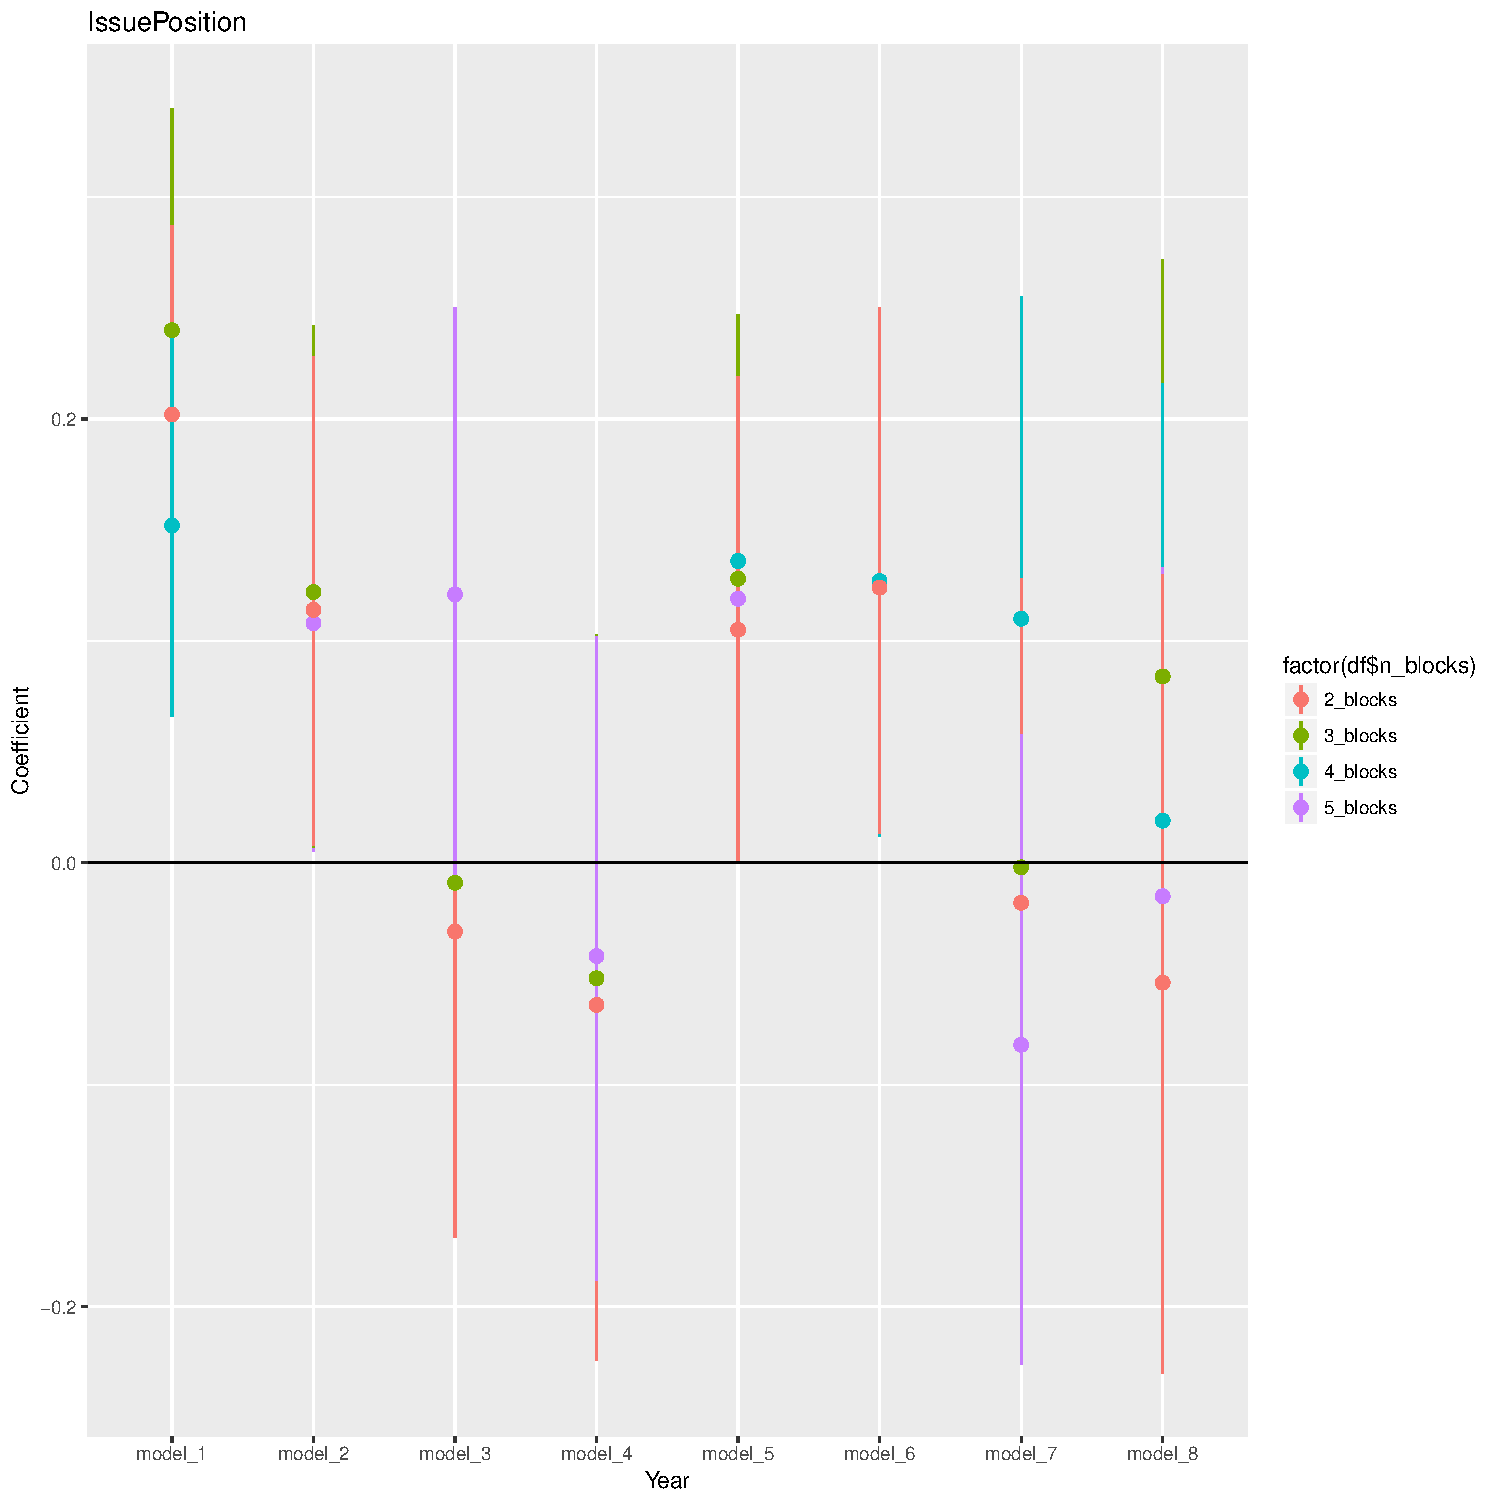
\includegraphics[height=.75\textheight, clip=true, trim=.5cm .5cm 0cm .6cm]{figures/rl_plots2/IssuePosition.pdf} \\
\caption{\label{fig:SBM_plot_pref} SBM covariate plot. Results from models for which DIC could not be calculated were discarded.}
\end{longtable}

\clearpage
\begin{longtable}[!h]{c@{\hskip 0cm}c}
Government alter \\
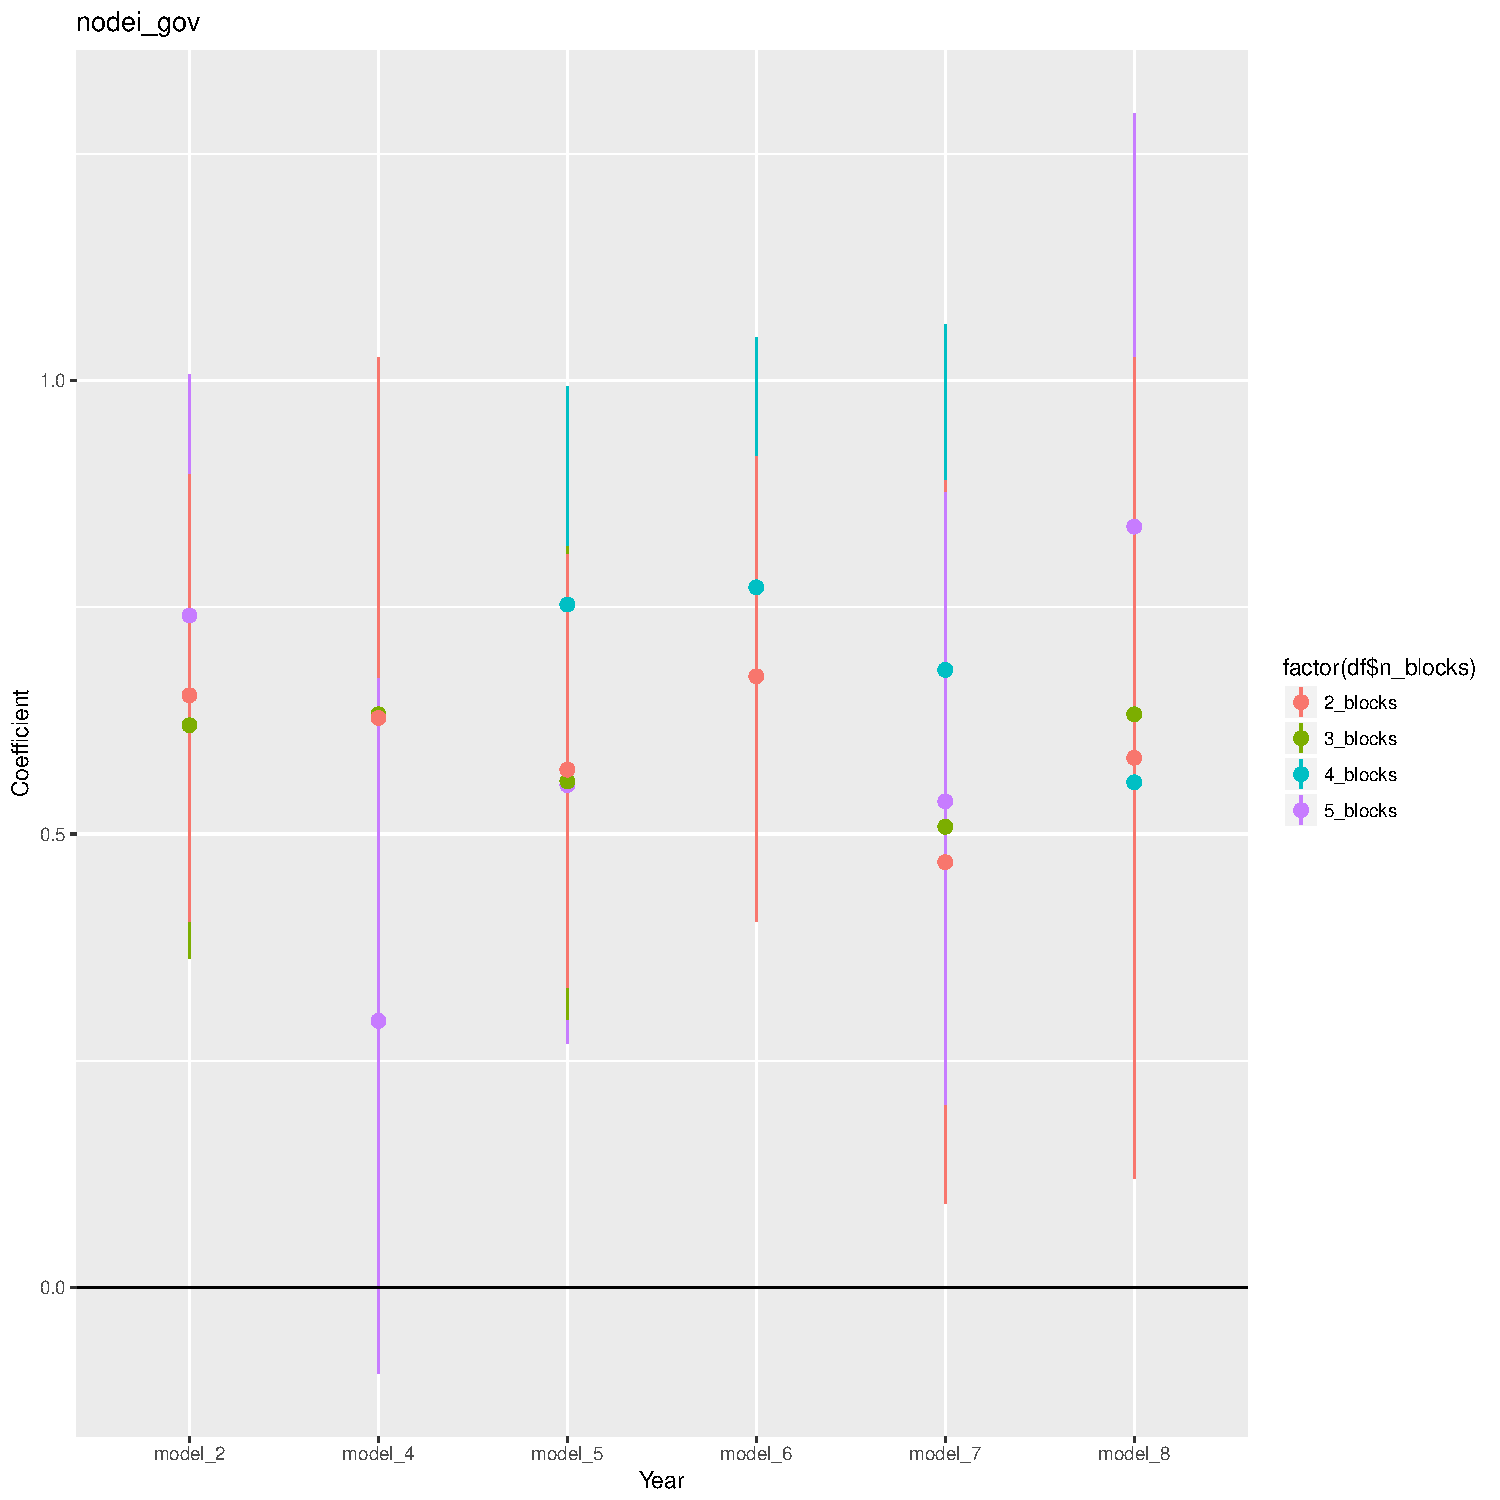
\includegraphics[height=.75\textheight, clip=true, trim=.5cm .5cm 0cm .6cm]{figures/rl_plots2/nodei_gov.pdf}   \\
\caption{\label{fig:SBM_plot_gov} SBM covariate plot. Results from models for which DIC could not be calculated were discarded.}
\end{longtable}

\clearpage
\begin{longtable}[!h]{c@{\hskip 0cm}c}
Scientific Ego \\
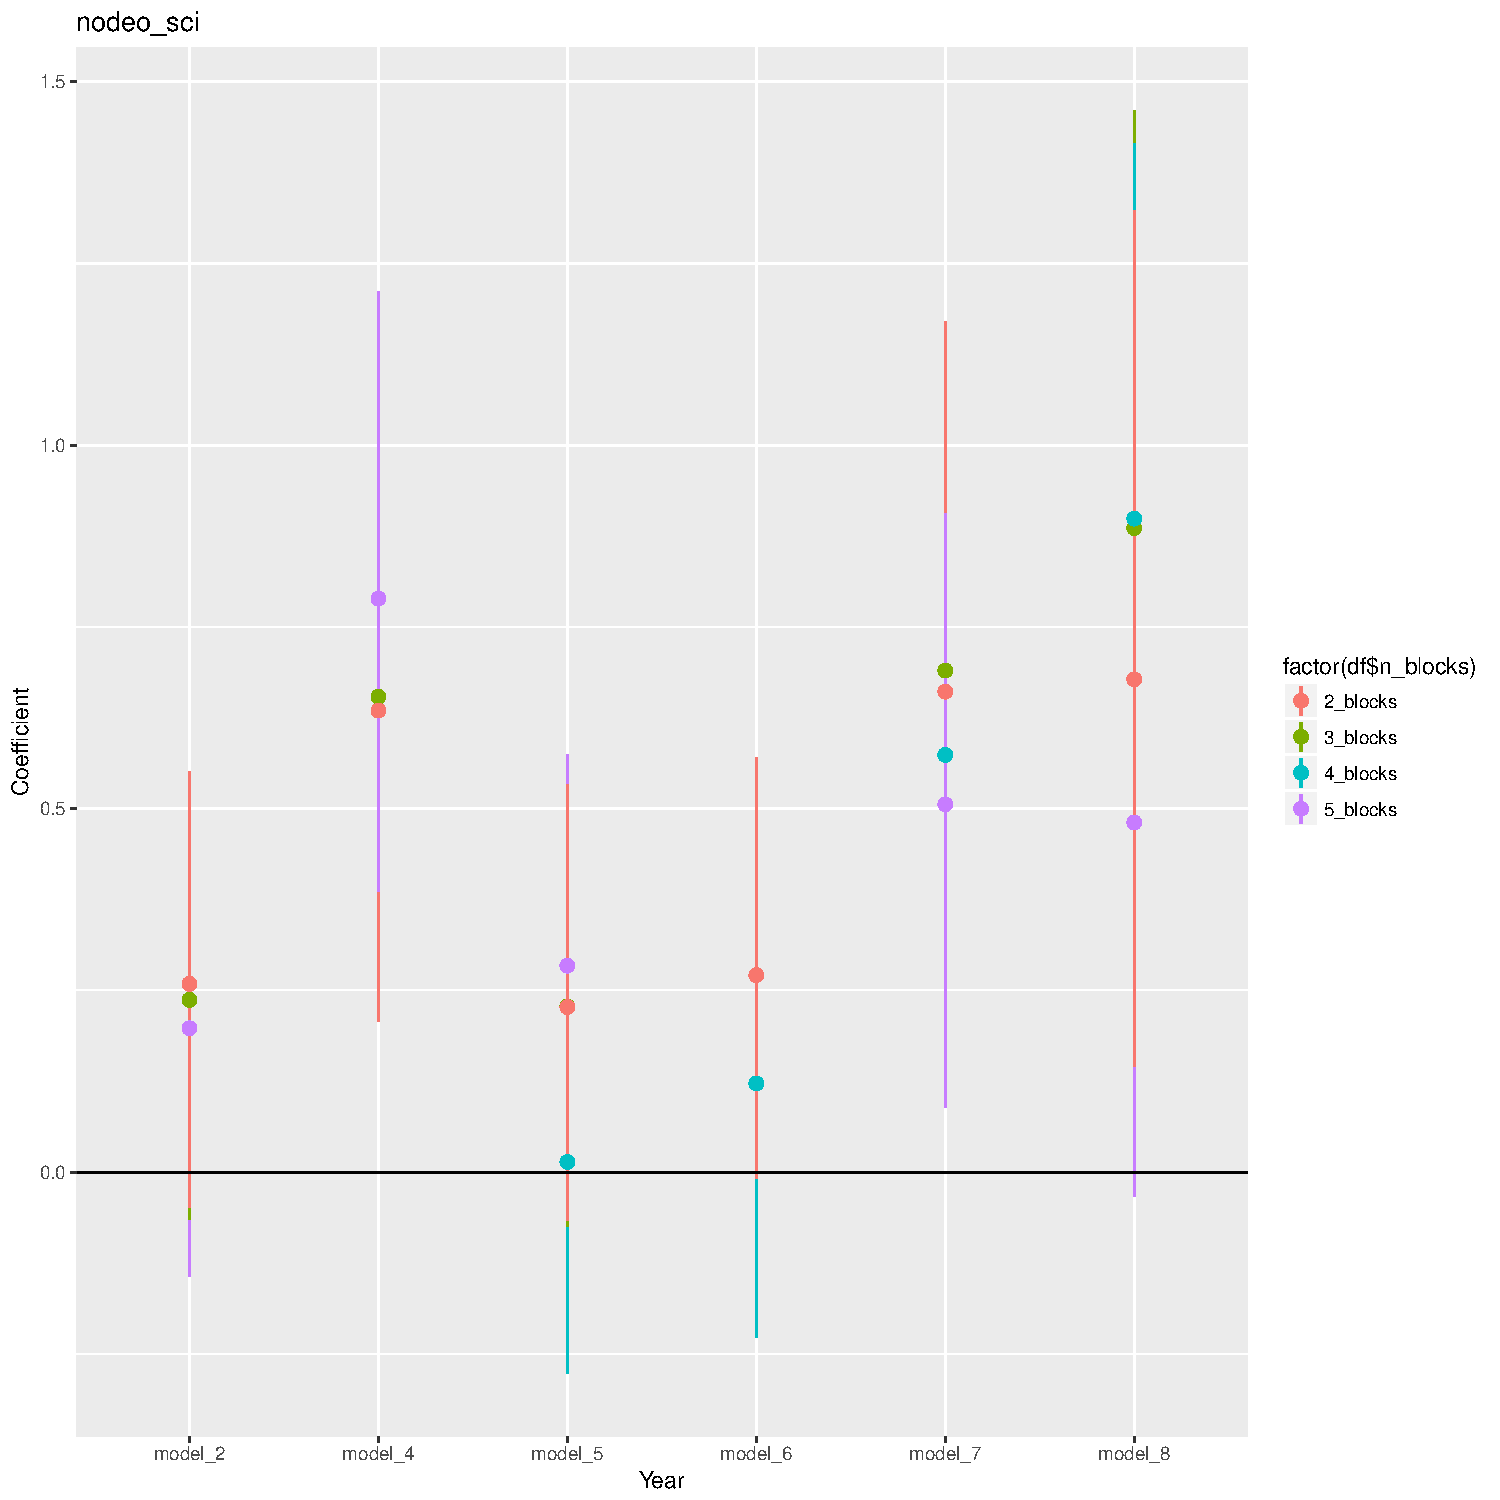
\includegraphics[height=.75\textheight, clip=true, trim=.5cm .5cm 0cm .6cm]{figures/rl_plots2/nodeo_sci.pdf}   \\
\caption{\label{fig:SBM_plot_sci} SBM covariate plot. Results from models for which DIC could not be calculated were discarded.}
\end{longtable}

\clearpage
\begin{longtable}[!h]{c@{\hskip 0cm}c}
Common Committee \\
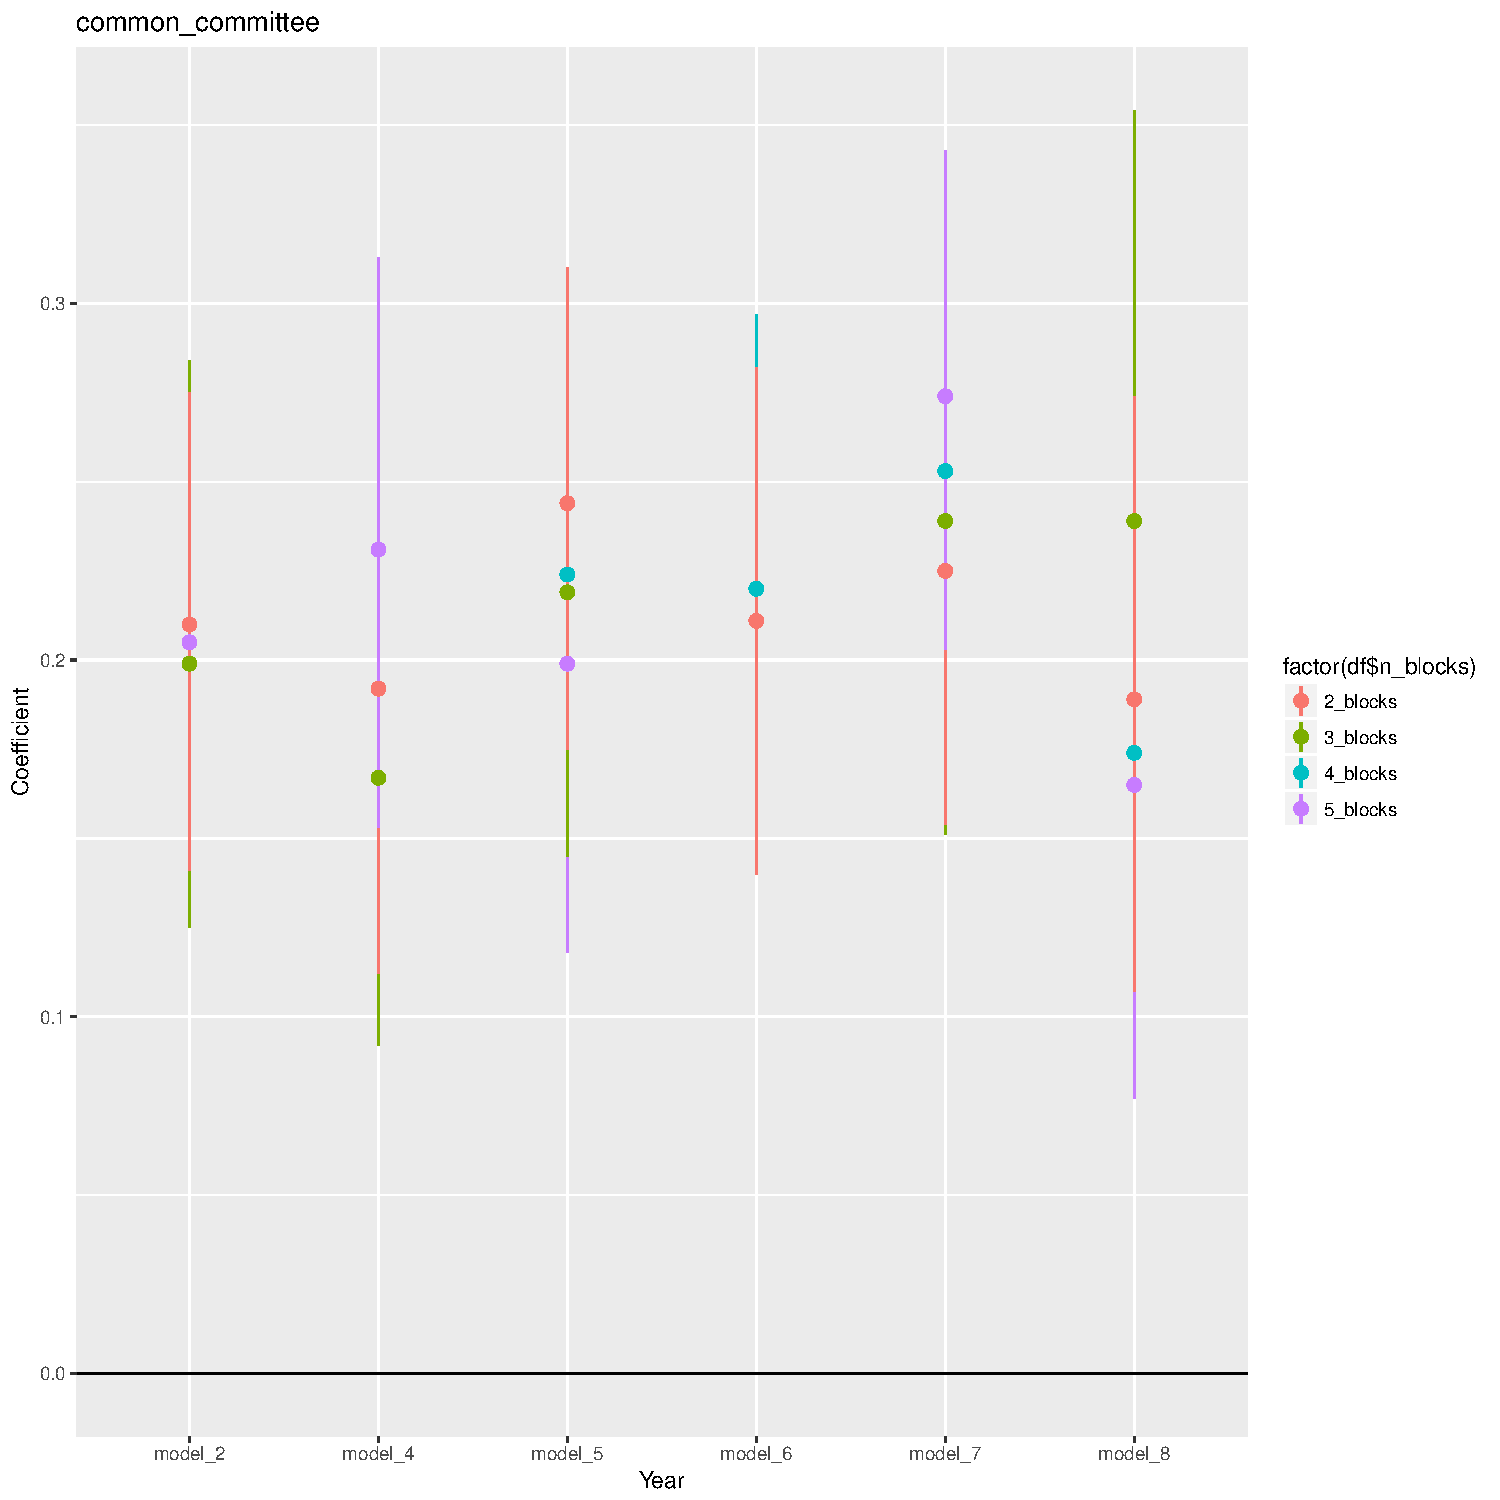
\includegraphics[height=.75\textheight, clip=true, trim=.5cm .5cm 0cm .6cm]{figures/rl_plots2/common_committee.pdf}   \\
\caption{\label{fig:SBM_plot_com} SBM covariate plot. Results from models for which DIC could not be calculated were discarded.}
\end{longtable}

\clearpage
\begin{longtable}[!h]{c@{\hskip 0cm}c}
Scientific Communication \\
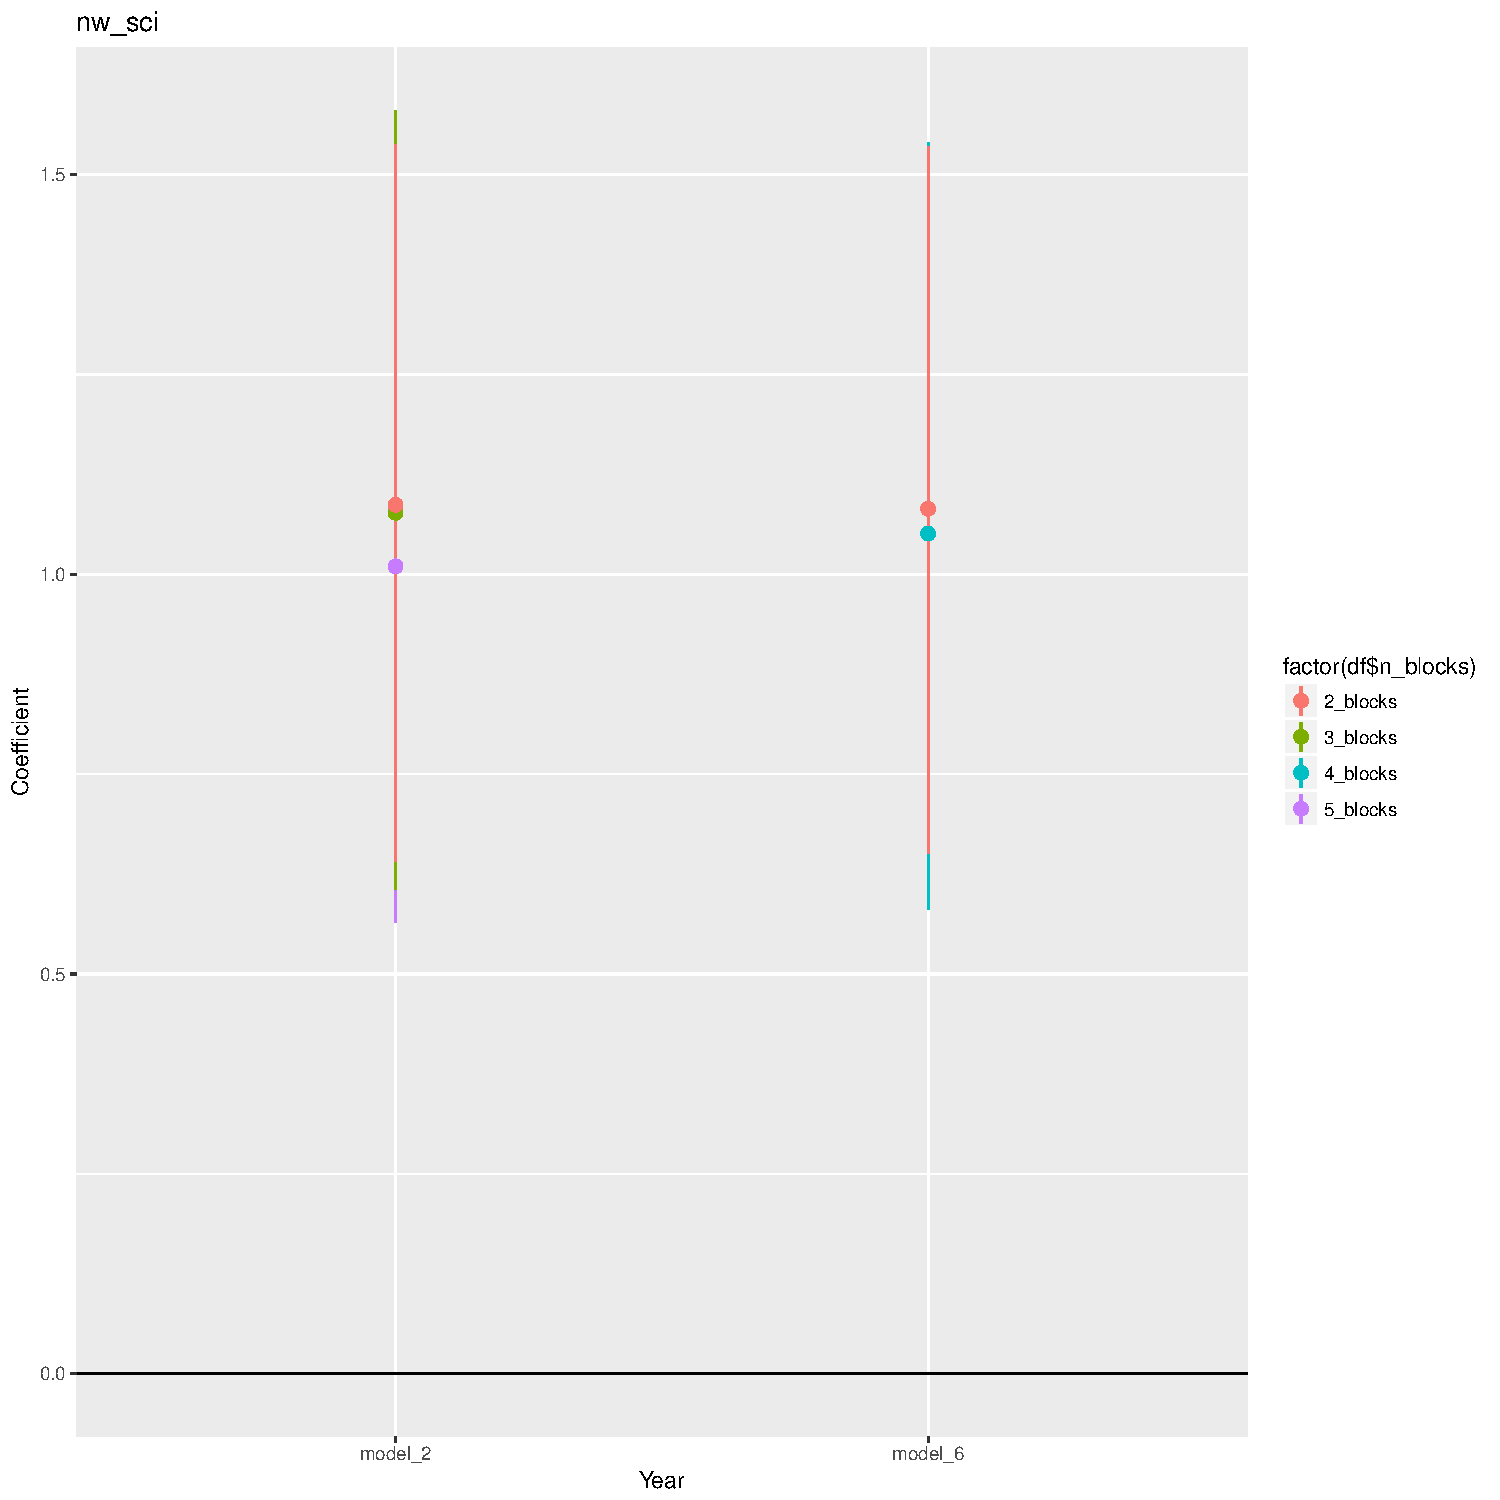
\includegraphics[height=.75\textheight, clip=true, trim=.5cm .5cm 0cm .6cm]{figures/rl_plots2/nw_sci.pdf}   \\
\caption{\label{fig:SBM_plot_nwsci} SBM covariate plot. Results from models for which DIC could not be calculated were discarded.}
\end{longtable}

\clearpage
\begin{longtable}[!h]{c@{\hskip 0cm}c}
Political Communication \\
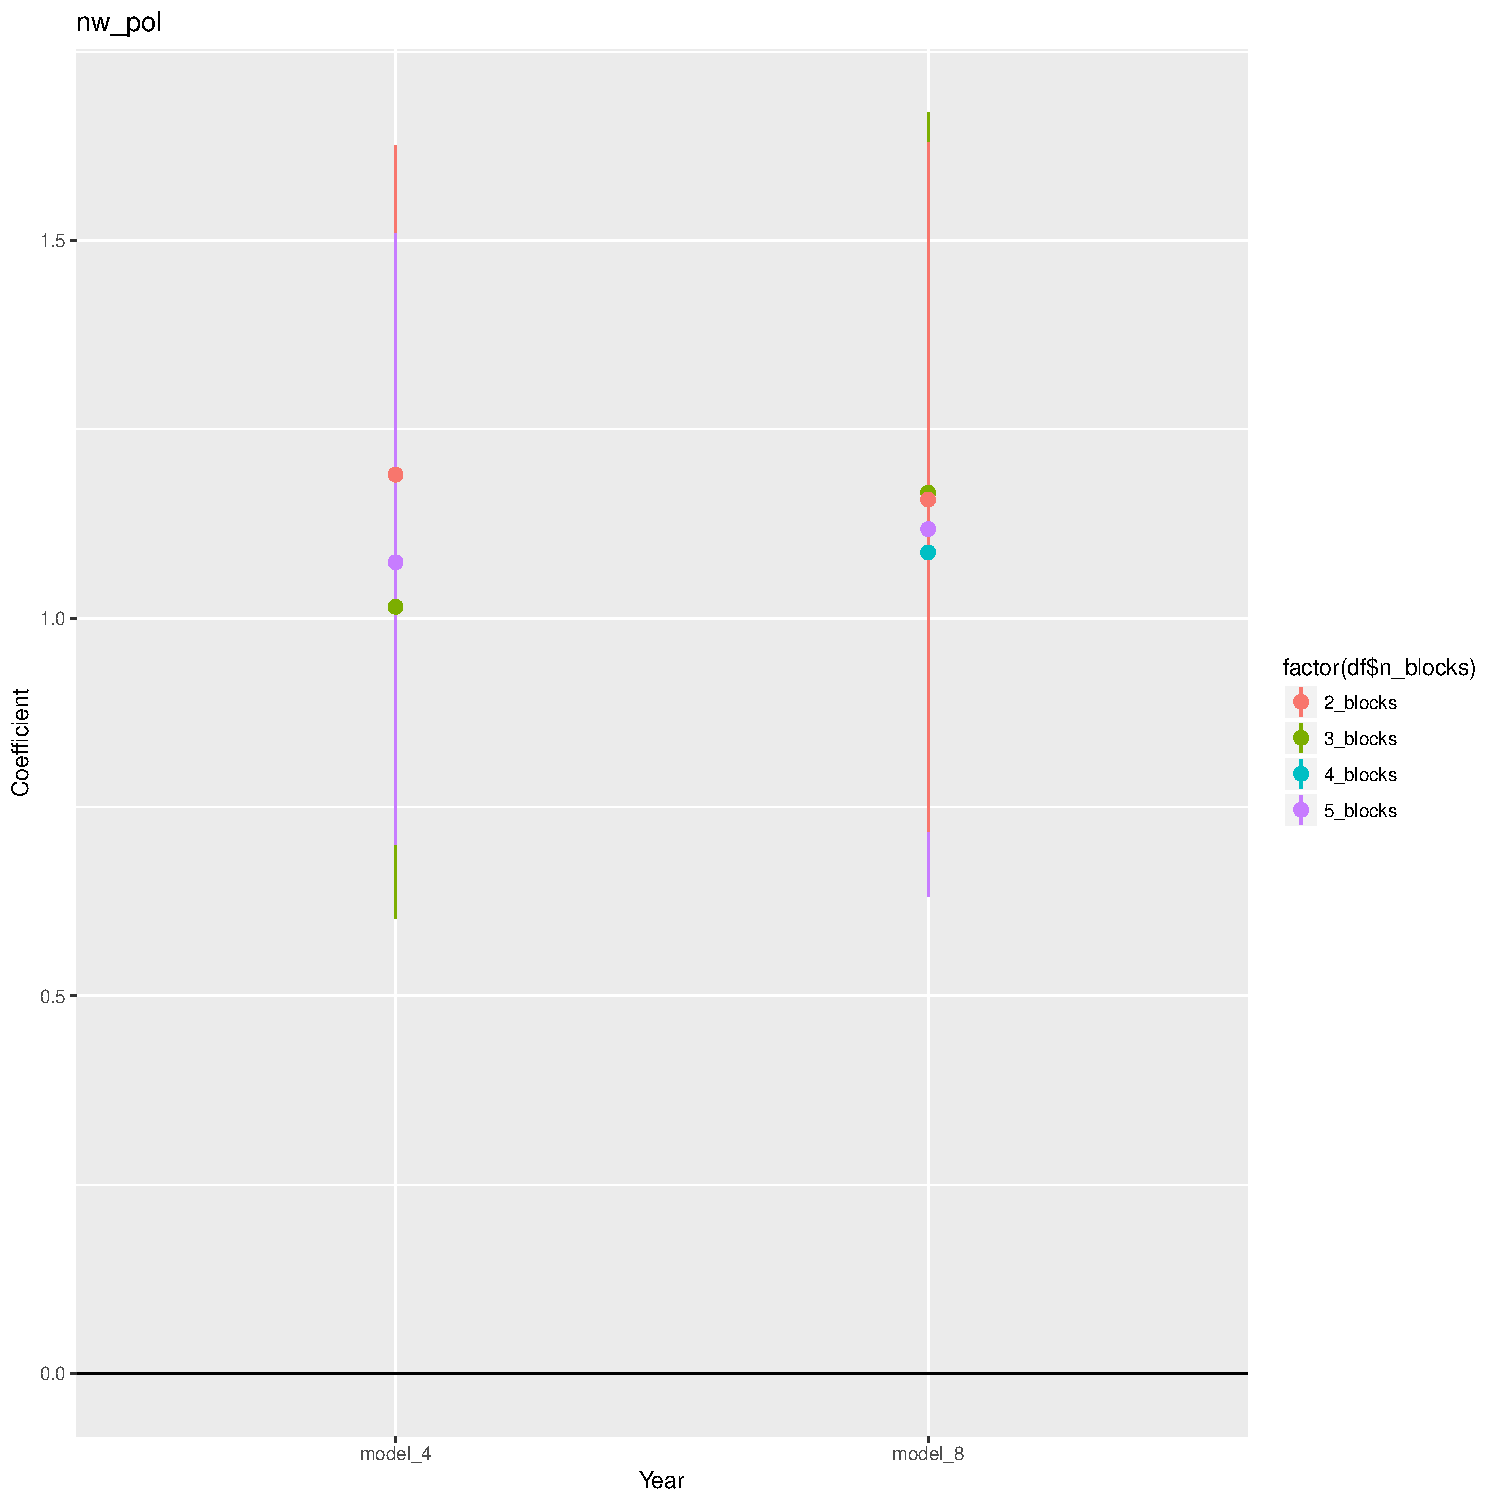
\includegraphics[height=.75\textheight, clip=true, trim=.5cm .5cm 0cm .6cm]{figures/rl_plots2/nw_pol.pdf}   \\
\caption{\label{fig:SBM_plot_nwpol} SBM covariate plot. Results from models for which DIC could not be calculated were discarded.}
\end{longtable}

\clearpage
\begin{longtable}[!h]{c@{\hskip 0cm}c}
Interest Group Homophily \\
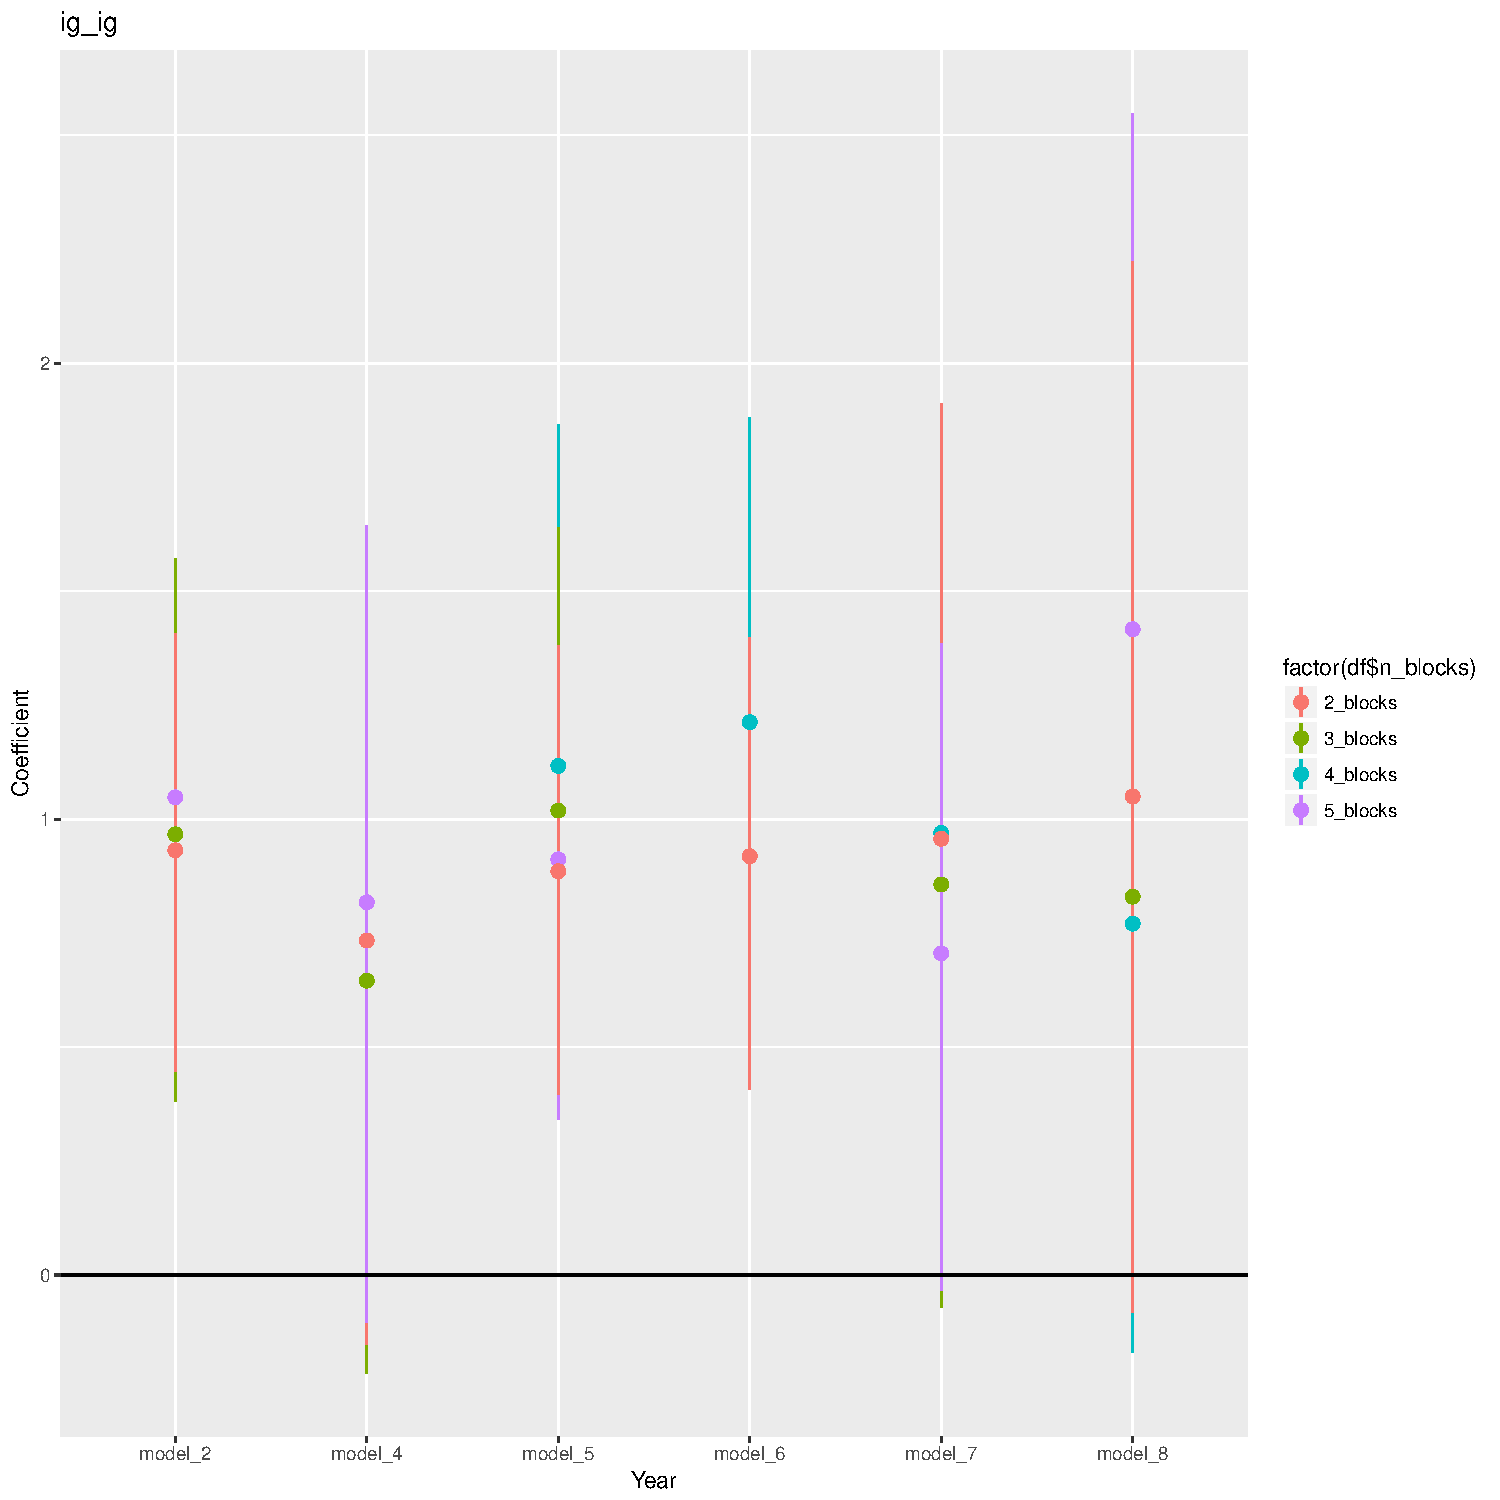
\includegraphics[height=.75\textheight, clip=true, trim=.5cm .5cm 0cm .6cm]{figures/rl_plots2/ig_ig.pdf}   \\
\caption{\label{fig:SBM_plot_igig} SBM covariate plot. Results from models for which DIC could not be calculated were discarded.}
\end{longtable}

\clearpage
\begin{longtable}[!h]{c@{\hskip 0cm}c}
Influence Attribution \\
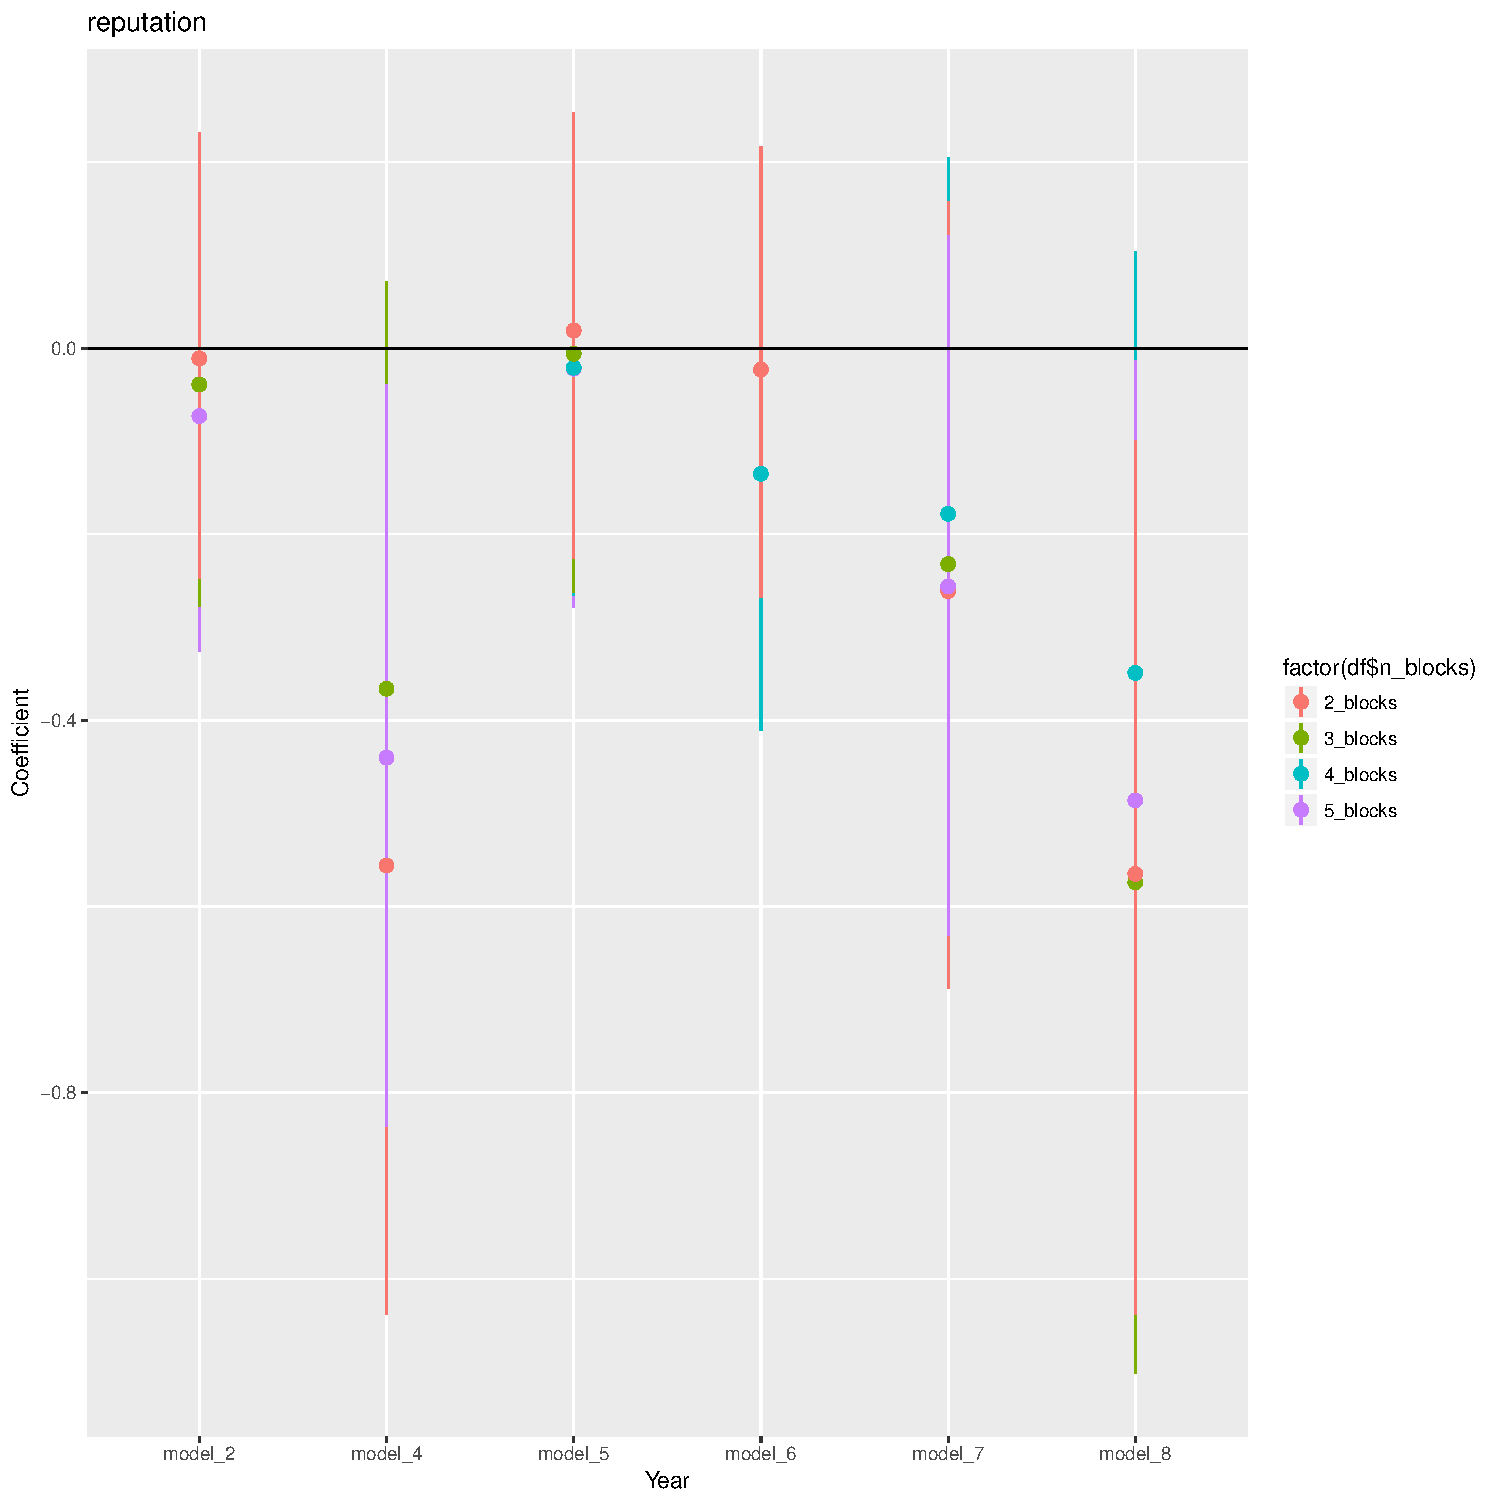
\includegraphics[height=.75\textheight, clip=true, trim=.5cm .5cm 0cm .6cm]{figures/rl_plots2/reputation.pdf}   \\
\caption{\label{fig:SBM_plot_reputation} SBM covariate plot. Results from models for which DIC could not be calculated were discarded.}
\end{longtable}

\clearpage
\begin{longtable}[!h]{c@{\hskip 0cm}c}
Betweenness \\
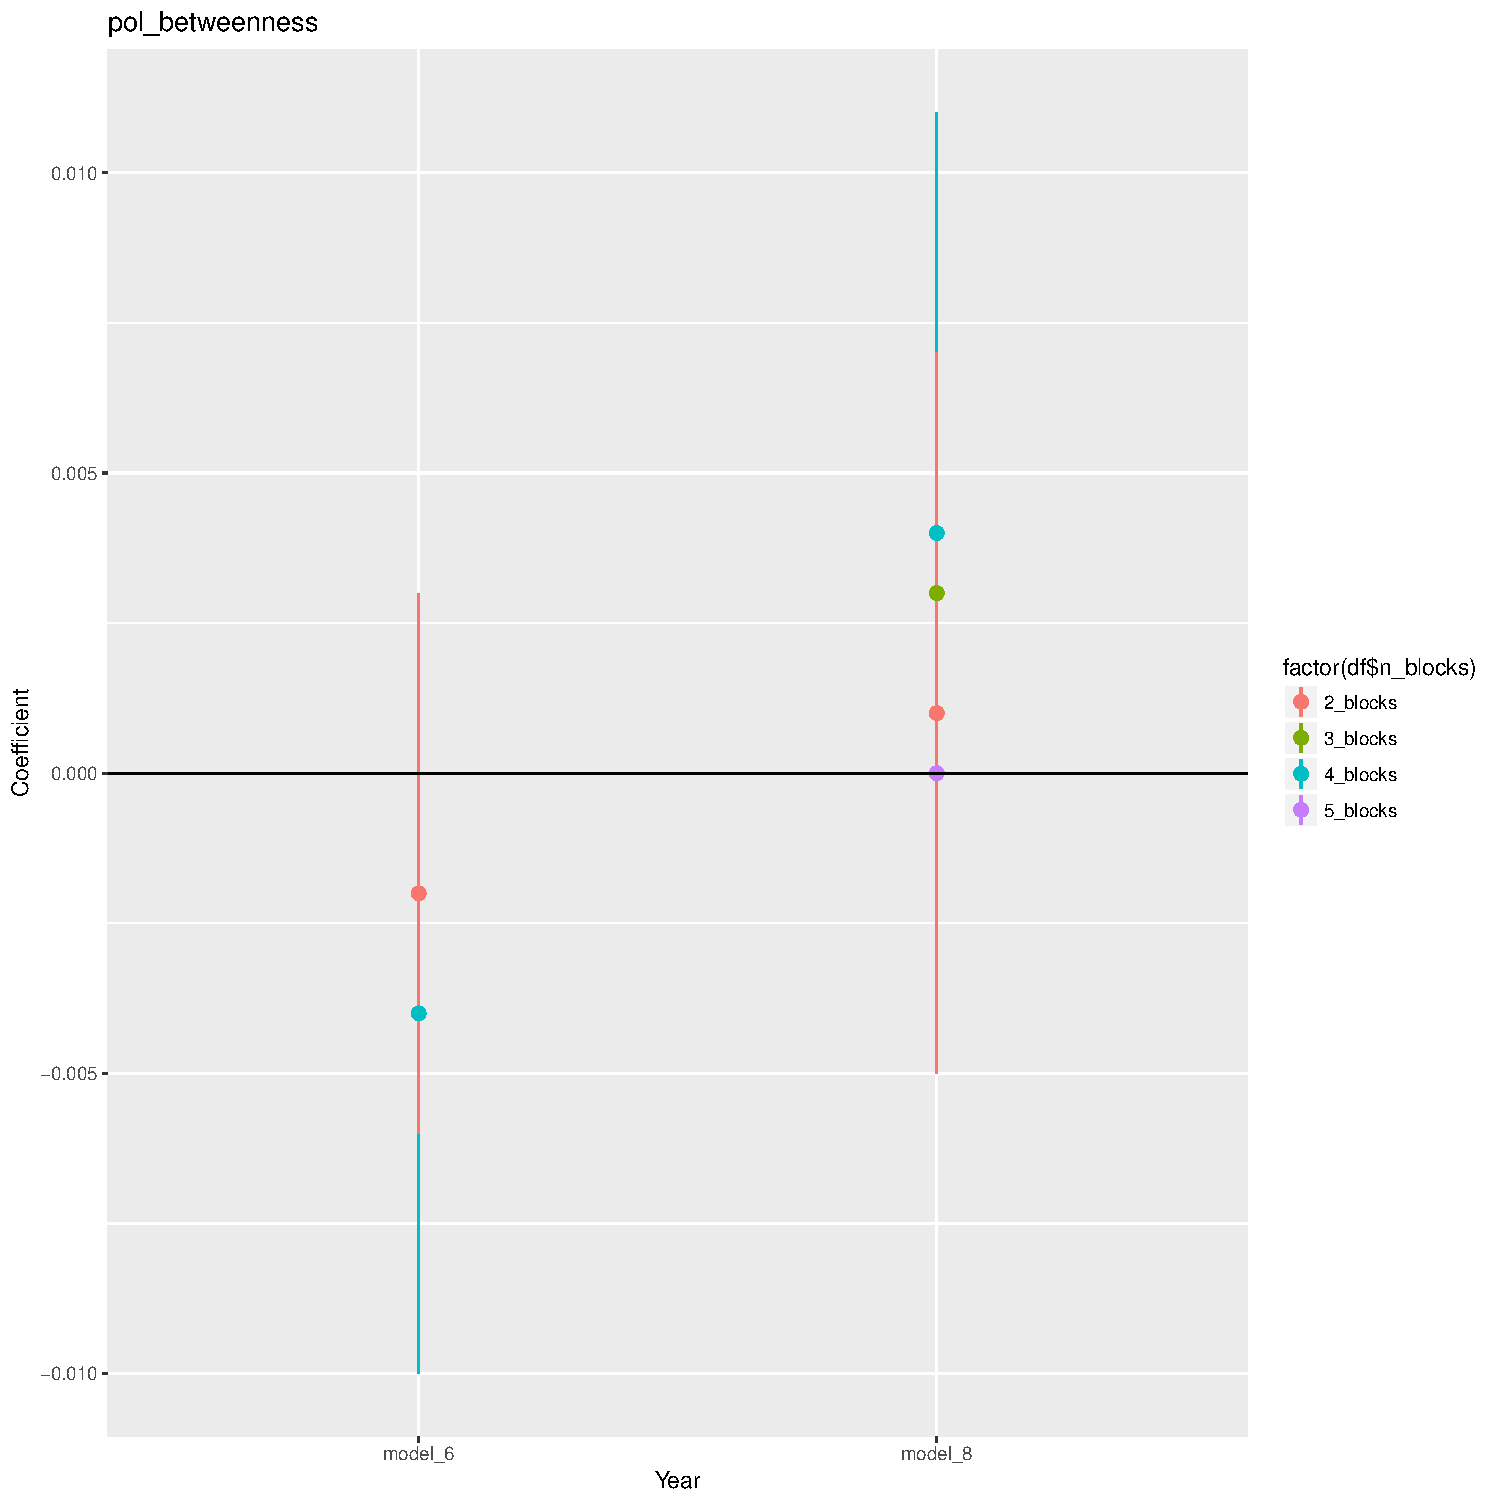
\includegraphics[height=.75\textheight, clip=true, trim=.5cm .5cm 0cm .6cm]{figures/rl_plots2/pol_betweenness.pdf}   \\
\caption{\label{fig:SBM_plot_between} SBM covariate plot. Results from models for which DIC could not be calculated were discarded.}
\end{longtable}



\subsection{Model Comparison}

\textbf{I only compare models one through four, as models five through eight are not reported in the main paper and are merely robustness tests. I included the results though above so that we could still review them and take them out later if we need too.}


\begin{enumerate}

\item ERGM replication
\begin{enumerate}
\item Models two and four do not perfectly replicate. Most of the substantive findings remain, but in model four the significance level for common committee drops from 99.9\% to 95\%. There are a few other drops in significance for other covariates, but not as big. Signage remains the same for the replication across all models even when there are changes in the coefficient size or significance. 
\end{enumerate}


\item LSM
\begin{enumerate}
\item There are substantial differences between the ERGM results and the LSM results. For example, in model 1, LSM does not have significant correlation between preference similarity and political communication. In model 2 the point estimate for common committee is five times larger  and  is not significant in model 4. Influence attribution is almost two times larger in model 2 and 4. In the LSM models, intercept estimates are not significant in any model, but they are highly significant in the ERGM models. Interest group homophily is not significant in model 4.
\end{enumerate}

\item SBM
\begin{enumerate}
\item Preference Similarity: In model 2, point estimates remain above 95\% significance cutoff. The variables for model 2 do not absorb preference similarity measures as they do in the ERGM.  
\item Government Alter: Point estimates are a little higher and in model 4 it is not 95\% significant for five blocks. 
\item Scientific Ego: Still statistically significant in model 4, but point estimates are less than half. 
\item Common Committee: Point estimate is about two thirds for model 2's and slightly bigger than model 4's.
\item Scientific Communication: Point estimate in model 2 is about $1/3$
\item Political Communication: Point estimate in model 4 is about $1/3$
\item Interest Group Homophily: Point estimates are slightly smaller and in model 4 they are not significant at the 95\% threshold. 
\item Influence attribution: point estimates are negative and not statistically significant instead of being around one. 
\item The number of blocks that results in the lowest DIC is not consistent across models. For the most part, models with four blocks have the lowest DIC for political communication but two blocks is best for scientific communication. Many of the institutional/relational structure variables are smaller not always significant at the same level.

\end{enumerate}
\end{enumerate}



\bibliographystyle{apsr}
\bibliography{bibliography}




\end{document}